\documentclass{article}

\usepackage[utf8]{inputenc}

\usepackage{natbib}
\usepackage{hyperref}
\usepackage[pdf]{graphviz}
\usepackage{graphicx}
\usepackage{amsmath}

\usepackage[colorinlistoftodos]{todonotes}

\usepackage{parskip}
\setlength{\parskip}{10pt} 

\usepackage{tikz}
\usetikzlibrary{arrows, decorations.markings}

\usepackage{chngcntr}
\counterwithout{figure}{section}

\begin{document}

\begin{titlepage}

\centering
  
{\scshape\LARGE Master thesis project proposal\\}
  
\vspace{0.5cm}
  
{\huge\bfseries E-graphs modulo theories\\}
  
\vspace{2cm}
  
{\Large Sofia Brookie \\ \href{mailto:sofia.ma@protonmail.com}{sofia.ma@protonmail.com} \\}
  
\vspace{1.0cm}
  
{\large Suggested Supervisor at CSE: Nicholas Smallbone\\}
  
\vspace{1.5cm}
  
{\large Relevant completed courses:\par}
  
{\itshape TIN093 Algorithms \\  DAT060 Logic in computer science \\}
  
\vfill

\vfill
  
{\large \today\\} 

\end{titlepage}

\section{Introduction}
E-graphs are a data structure and mechanism for automatically discovering and proving equations that hold
between a set of first-order terms, given as input a starting set of terms and a \textit{theory} (a set of identities). E-graphs were pioneered by Nelson and Oppen \cite{nelson1980fast}, but have seen an explosion of interest much more recently with the \textsc{Egg} library developed by Willsey et al. and their corresponding paper \cite{willsey2021egg}. This paper developed several techniques for
significantly improving the ergonomics and speed of e-graph-based proving, and applied it
to a diverse set of research problems: improving the accuracy of floating-point computations, optimizing linear algebra kernels, and decompiling 3D computer-assisted-design models into structured, generalizable programs.

However, e-graphs struggle with the combinatorial explosion involved in directly reasoning about certain theories, such as those containing associative and commutative operators. Despite the existence of well-known techniques to reason about associative and commutative operators, standard e-graphs handle use generic mechanisms to reason about theories containing these operators in a subtheory, resulting in a potential exponential expansion in the e-graph size just to deduce basic consequences of the associative and commutative identities.

Zucker \cite{zucker2025omelets} proposes extending the notion of e-graphs to that of \textit{E-graphs Modulo Theories} (EMTs) in order to use much more efficient techniques to handle associative and commutative subtheories, and use the e-graph mechanisms only for the other identities in the theory. They also suggest other subtheories for which EMTs can make reasoning more efficient by using standard theory-specific techniques, such as the handling the theory of vector spaces with Gaussian elimination.

Working with e-graphs modulo theories requires \textit{matching modulo theories}, for which Zucker presents a simple algorithm they refer to as the \textit{bottom-up algorithm}. Our goal is to elaborate on this algorithm, to describe the matching modulo theories problem more generally, and to situate the bottom-up algorithm within a family of matching algorithms. We then aim to implement some of this family of matching algorithms and compare the performance with standard e-graph methods.

\section{Background}

\subsection{Equational theorem proving preliminaries}
In general, we will have some set of \emph{function symbols}, say, $f$ and $g$, and some \emph{identities}, such as $f(a, b) = g(f(a, b))$, where throughout the text, $a$, $b$, and $c$ will be the variables appearing in identities; the meaning of an identity is that it holds for any value of these variables. This is the background \emph{theory}. We will take the theory and apply it to a set of terms, say, $\{x, f(x, g(y)), g(f(x, g(y)))\}$. We will use $x$, $y$, $z$, and $w$ as variables in terms; they are not explicitly logically quantified, but are algebraic indeterminates; they can be thought of as 0-ary function symbols satisfying no laws. Applying the theory to a set of terms, we can discover new equations, such as $f(x, g(y)) = g(f(x, g(y)))$ in our small example here. E-graphs are a systematic method to determine equations among a set of terms given a background theory; we say an e-graph is \emph{saturated} if it represents all equations among the input terms, and there is nothing less to discover.

An e-graph is a graph where each node is an equivalence class (e-class) of terms, with the edges representing how one equivalence class can be represented as a function symbol applied to other equivalence classes. In particular, we can think of a node $n$ as containing a set of terms along the lines of $\{f(n, m), \ldots, g(o)\}$: function symbols applied to the names of other nodes, which are the same as edges pointing to other equivalence classes of terms. In this way, e-graphs naturally represent congruence: if functions have equal arguments, they have equal results. As long as certain invariants are maintained, arguments to functions are only references to the equivalence classes of those arguments, so congruence over these equivalence classes is a direct consequence of the representation.

\subsection{Motivation: associativity and commutativity}
Some common mathematical identities in theories that e-graphs are expected to handle include
associativity ($f(a, f(b, c)) = f(f(a, b), c)$) and commutativity ($f(a, b) = f(b, a)$). While e-graphs are able to handle any set of identities, associativity and commutativity lead to an explosion in the size of the e-graph when it is saturated, as the number of equivalence classes of subterms of a term with $n$ occurences of an associative and/or commutative function is proportional to $\exp(n)$. Even if applying identities stops before saturation,
it is likely that a large number of `useless' associativity/commutativity steps will have been taken.

We will show some examples of e-graphs handling associativity and commutativity for a function called `Add', on input terms of increasing size. We will also use the binary operator $+$ as the function symbol for `Add'. We use the online Egglog demo \cite{egglogdemo} to apply the rules and generate the resulting e-graph.
In the smallest example (Figure \ref{egxz}), using just the term $x + z$, the e-graph will run to saturation, and
give us three equivalence classes: $\{x\}$, $\{z\}$, and $\{x + z, z + x\}$.

\begin{figure}[!ht] % suggests placing the figure here
    \centering % Centers the figure in the column
    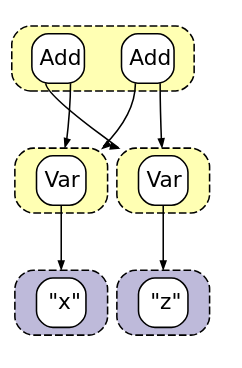
\includegraphics[width=0.3\columnwidth]{addxz}
    \caption{E-graph of the term $x + z$ after rewriting to saturation.}
    \label{egxz}
\end{figure}

Each yellow box is an equivalence class of terms that the e-graph algorithm has discovered by applying identities, and each white node inside a yellow box is the root function of one of the equivalent terms.

The process is to add the input terms to the graph. Then, we \emph{match} either the left-hand or right-hand side of an identity to the graph. In our example, we match $a + b$ to $x + y$ in the natural way. Then we add a term for the other side of the equation to the graph, and merge the resulting node with our original one to represent that they are equal. In this case, the we have $x + z$ matching the left-hand side of the identity $a + b = b + a$, so we add the term $z + x$ to the graph, and merge its equivalence class with that of $x + z$. We can then apply the identity to our newly-added term, but no more \emph{new} nodes or equalities result, so we have reached saturation.

If we consider the larger term $x + (y + z)$ (Figure \ref{egxyz}), there are several more equivalence classes, and the associativity rule is applied for the first time. We get one equivalence class each for all three of $\{x+y,y+x\}$, $\{y+z,z+y\}$ and $\{z+x,x+z\}$, as well as a six-item equivalence class of all the ways to commute and associative the input term: for instance, the rightmost node in the top equivalence class itself points to the equivalence class $\{x+y,y+x\}$ as its first argument, so it represents the set of terms
$\{(x+y)+z, (y+x)+z\}$. The e-graph representation allows some compactness in that each of the nodes in the top class represent two equivalent terms each, letting us represent 12 equivalent terms with only 6 nodes, but this isn't sufficient to stop the exponential increase in the e-graph size when we increase the size of the term.

\begin{figure}[!ht] % suggests placing the figure here
    \centering % Centers the figure in the column
    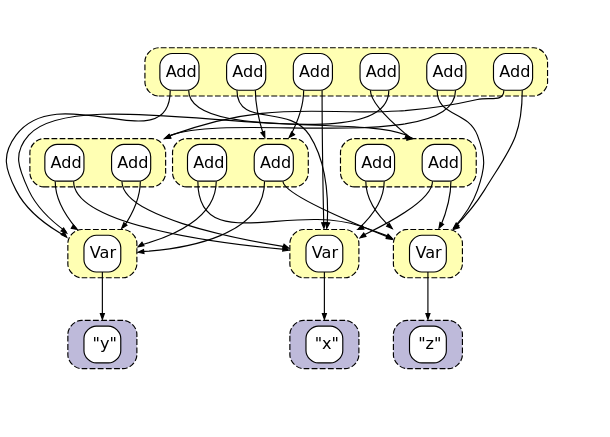
\includegraphics[width=\columnwidth]{addxyz}
    \caption{E-graph of the term $x + (y + z)$ after rewriting to saturation.}
    \label{egxyz}
\end{figure}

If we enter the term $x + ((y + z) + w)$ into the demo (Figure \ref{egxzw}), the resulting e-graph
is not even saturated, but the size has increased to the point where we reach the demo's built-in limit.

\begin{figure}[!ht] % suggests placing the figure here
    \centering % Centers the figure in the column
    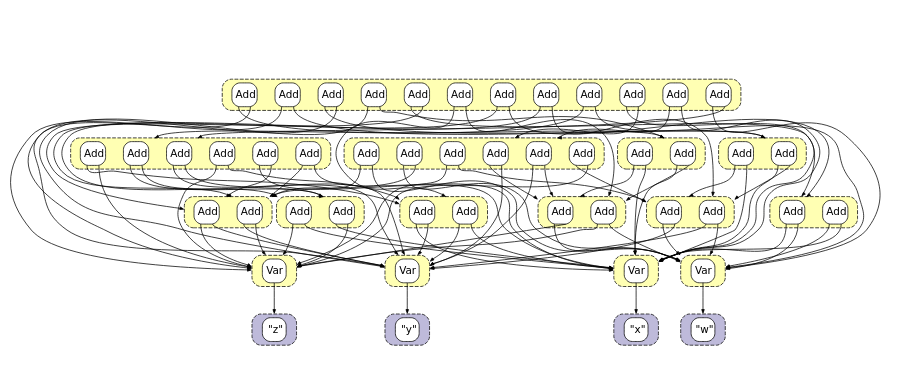
\includegraphics[width=\columnwidth]{add}
    \caption{E-graph of the term $x + ((y + z) + w)$ after a number of rewriting steps.}
    \label{egxzw}
\end{figure}

This graph shows that typically there are many syntactically-distinct terms that are equal modulo associativity and commutativity, which makes each equivalence class big, but also that there are many inequivalent \textit{subterms} that are referenced by the equivalence class of the input term.

The \textsc{Egg} library handles the application of identities with a backoff method, where
equations to apply are selected based on their weight, and the weight of an equation decreases when it fires. Any equation that suffers from blowup, like associativity or commutativity, will be fired less and less, in the hopes of finding more `interesting' equalities without having to run to saturation. This method isn't able to properly distinguish between `interesting' and `uninteresting' cases of associativity and commutativity, and it's also of no use when running to saturation.

In the rest of the paper, we will use `A/C' to refer to associativity and/or commutativity; namely, each of the three theories `A', `C', and `AC'. The theories are related, but each is independently useful.

To give an example of a theory with both A/C and `interesting' equalities, we extend the theory from above (containing only the function Add and the AC equations) with a function $f$, satisfying $f(a + b) + 1 = f(a) + f(b)$. We also allow integer constants, and allow the e-graph to reason about integer arithmetic, e.g. that $1+1=2$. We begin with the term $f(x) + (f(y) + f(z))$. We would like to discover that this input term is equal to $f(x + (y + z)) + 2$, using the reasoning

\begin{align*}
	&f(x) + (f(y) + f(z)) = \\
	&f(x) + (f(y + z) + 1) = \\
	&(f(x) + f(y + z)) + 1 = \\
	&(f(x + (y + z)) + 1) + 1 = \\
	&f(x + (y + z)) + (1 + 1) = \\
	&f(x + (y + z)) + 2
\end{align*}

As we can see in Figure \ref{egf1}, the e-graph is on the way to discovering this, having for instance generated an equivalence class for the constant $2$, but hits the demo's limit again before completing this proof. While this example may be a toy example on a rather limited demo, it shows the extent to which A/C can clutter up the e-graph with many nodes that are not essential to a desired proof. Our equational proof above only needs to use associativity twice.

\begin{figure}[!ht] % suggests placing the figure here
    \centering % Centers the figure in the column
    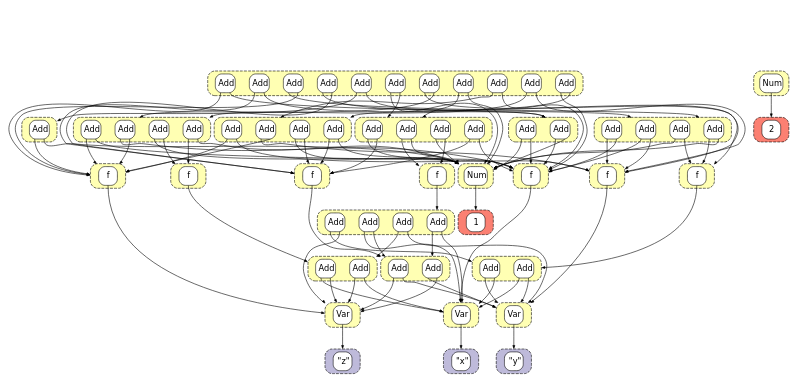
\includegraphics[width=\columnwidth]{addf1xyz}
    \caption{E-graph of the term $f(x) + (f(y) + f(z))$ after a number of rewriting steps.}
    \label{egf1}
\end{figure}

One could attempt to deal with AC ahead-of-time by automatically generating derived equations like $f(a+b) + (1 + c) = (f(a) + f(b)) + c$ and $1 + f(a+b) = f(a) + f(b)$ from the source equation. This method is not in general complete: in the AC case, we would need infinitely many equations to handle matching at an arbitrary distance, as we can see with the term
$f(x+y) + (z_1 + (z_2 + \ldots (z_n + 1) \ldots))$. Here, any pattern that can determine that both $f(x+y)$ and $1$ are subterms, and therefore that there is a match modulo AC, must have $n$ auxiliary variables to capture (and ignore) each $z_n$ that stand between the $f(x+y)$ and the $1$.

This gives some idea of the difficulty in simply preprocessing the input theory and set of terms, and motivates considering a modification to the e-graph representation and algorithms themselves.

\subsection{Prior work on reasoning modulo theories}
There have been various proposals to alter the e-graph algorithms to, at least partially, solve the exponential size problem for A/C and similarly problematic theories. We focus on the paper at \textsc{Egraphs} 2025 by Zucker \cite{zucker2025omelets}, which introduces the notion of E-graphs Modulo Theories. The name is inspired by \emph{Satisfiability Modulo Theories} (SMT) solvers, which have seen significant improvements in speed and capabilities in recent decades. SMT solvers don't precisely solve
the same problems as e-graphs, but there is significant overlap in that they are both methods of theorem-proving in fragments of first-order logic. Modern SMT solvers use knowledge of a variety of built-in theories to solve input problems quickly.

The idea of E-graphs Modulo Theories is to take inspiration from SMT solvers and extend the e-graph mechanism with specific built-in theories. For example, as demonstrated above, the generic mechanisms of e-graphs handle A/C poorly, but there are methods to efficiently reason about terms modulo these identities.

The key differences between EMTs and standard e-graphs is that we now represent our graph \emph{modulo theories}, so that, say, a single node that in a standard e-graph would represent $x+(y+z)$ is now taken to represent the 12 equivalent re-ordered and re-associated terms modulo AC. In order to achieve this, we need two key ingredients: when adding nodes to a graph, we need to \emph{canonicalize} them to one of the equivalent terms, so that, say, if we add $x+y$ and $y+x$ they will be canonicalized to the same representing term and thus considered to be identical. Canonizers for a variety of theories are well-known, and mostly involve making particular choices, such as imposing an ordering on terms and choosing that association will canonically be to the right. The harder problem is \emph{matching modulo theories}.

As an example of matching modulo theories, consider the equation we introduced above: $f(a + b) + 1 = f(a) + f(b)$. If we consider AC to be a built-in theory, then, when we match this against the term
$f(x+y) + (1 + f(z))$, we need a way to automatically determine that this term is equivalent to $(f(x+y) + 1) + f(z)$, and so contains a subterm that matches the pattern; thus the original term can be rewritten to $(f(x) + f(y)) + f(z)$. Besides AC, we might, for instance, also consider matching modulo the laws of negation, so that $f(x+y)$ itself can be matched to the left-hand side, and rewritten to $(f(x) + f(y)) - 1$.

We need an algorithm that can do efficient and complete matching while taking into account the built-in theory. Zucker \citep{zucker2025omelets} provides a sketch of such an algorithm, which we will use in an example of working modulo theories.

First, we introduce our term $f(x) + (f(y) + f(z))$ (Figure \ref{egmt1}).

\begin{figure}[!ht] % suggests placing the figure here
    \centering % Centers the figure in the column
    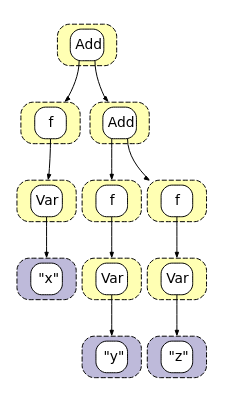
\includegraphics[width=0.3\columnwidth]{addmt1}
    \caption{E-graph of the term $f(x) + (f(y) + f(z))$ modulo AC}
    \label{egmt1}
\end{figure}

This term is canonized by an AC canonizer that right-associates terms and orders variables according to $x < y < z$.

Next, we match and apply three instances of the identity $f(a + b) + 1 = f(a) + f(b)$. Since we are working modulo AC, we don't need to match and extend the e-graph based on identities for associativity and commutativity, but we need to find matches of $f(a) + f(b)$ \emph{up to AC}. We can do this as follows: first, we list all possible substitutions for $a$ and $b$ that exist in our graph: we have 8 nodes, so there are 8 possibilities for both. Then, we filter both sets to narrow down to those e-classes that have $f$ as a parent, and thus find all possible e-classes matching $f(a)$ and $f(b)$. Then, we look for all e-classes containing `Add' that have one e-class matching $f(a)$ and one e-class matching $f(b)$ as \emph{indirect} children, and ignoring the order of the children. These conditions mean the match is modulo AC. This is a simple form of Zucker's bottom-up matching algorithm, and it is sufficient to find all 3 matches for the right-hand side of the identity in the initial graph.

Adding the substituted instances of the left-hand side of the identity to the graph, we get the following e-graph with 10 new e-classes (Figure \ref{egmt2})

\begin{figure}[!ht] % suggests placing the figure here
    \centering % Centers the figure in the column
    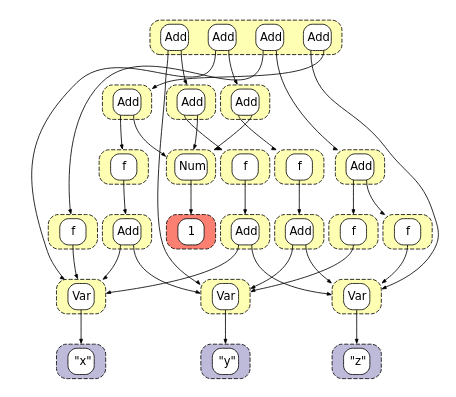
\includegraphics[width=0.8\columnwidth]{addmt2}
    \caption{E-graph of the term $f(x) + (f(y) + f(z))$ modulo AC after 1 rewriting step}
    \label{egmt2}
\end{figure}

We apply three more instances of the same identity, but these all generate the same new terms, so nothing changes (Figure \ref{egmt3}).

\begin{figure}[!ht] % suggests placing the figure here
    \centering % Centers the figure in the column
    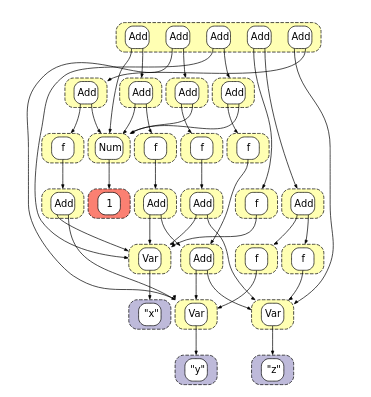
\includegraphics[width=0.8\columnwidth]{addmt3}
    \caption{E-graph of the term $f(x) + (f(y) + f(z))$ modulo AC after 2 rewriting steps}
    \label{egmt3}
\end{figure}

Finally, we use $1+1=2$ and reach saturation (Figure \ref{egmt4}).

\begin{figure}[!ht] % suggests placing the figure here
    \centering % Centers the figure in the column
    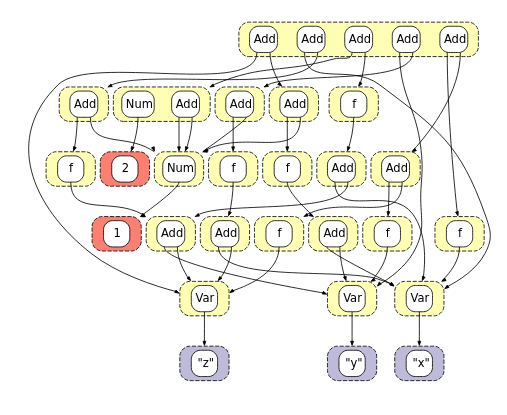
\includegraphics[width=0.8\columnwidth]{addmt4}
    \caption{E-graph of the term $f(x) + (f(y) + f(z))$ modulo AC after 3 rewriting steps, reaching saturation}
    \label{egmt4}
\end{figure}

We see that by working modulo AC, we reach saturation with only a few extra equivalence classes added, and no extra nodes to represent all the ways to commute and re-associate any uses of Add. Like with standard e-graphs, we are able to quickly discover the desired equality without any form of goal-directed search; we just need to run to saturation to discover all possible equalities from our input.

\subsection{Algorithms for matching (possibly modulo theories)}
E-graph matching is a core step in discovering new equalities between terms in the graph, but matching modulo theories in a traditional top-down way has inherently exponential time-complexity in certain cases, and as much as infinite time complexity in others. However, Zucker's bottom-up matching method can match in non-exponential and finite time, respectively. There is a trade-off, with the speed of bottom-up matching now dependent on factors that top-down-matching is not sensitive to.

The conceptual top-down/bottom-up distinction is based on whether matching proceeds bottom-up from the leaves of a tree representing a term, or top-down from the root.

Zucker proposes that there ought to be a `mixed top-down/bottom-up' approach which can perform optimally in a range of situations.

\textsc{Egg} uses the top-down-style Rete algorithm \cite{forgy1989rete}, which matches somewhat faster than a na\"ive top-down approach.

It is pointed out by Zhang et al. in \citep{zhang2021relational} that e-graph matching is simply a \textit{conjunctive query} over the term graph viewed as a relation, which can be solved by algorithms used in databases for computing joins. The recent work on
Worst-Case Optimal Join (WCOJ) algorithms \cite{ngo2018worst} provides algorithms that are asymptotically better join performance than traditional binary joins, and there is also work on Free Joins \cite{wang2023free}, which provide a spectrum of algorithms that trade off between the asymptotic optimally of WCOJs with the practical speed advantages of binary joins. Zhang et al. explore the application of WCOJ algorithms to e-graph matching, showing significant performance improvements over Rete's algorithm.

WCOJ algorithms do not have an inherent directionality. It is based on this work that Zucker suggests the possibility of a `mixed top-down/bottom-up' matcher for e-graphs modulo theories.

\section{Goals: understanding matching modulo theories}
\subsection{Goal 1: a new formulation of the join problem}
This goal is based on as-yet unpublished work I have done prior to the submission of this proposal.

The various algorithms for matching discussed fit into a framework of *join plans* where they can be expressed as rearrangements of the same underlying conjunctive query. To be more specific, conjunctive queries fit directly into the diagrammatic language of string diagrams over monoidal categories \citep{selinger2010survey}, which I aim to use as a clarifying way to formulate the different `directions' of matching and the asymptotic tradeoffs. This is an extension and formalization of the syntax for various join plans given in the paper on Free Joins \cite{wang2023free}.

This formulation is clarifying but not trivial, in the sense that there are different performance costs to the various ways of expressing a conjunctive query despite them being algebraically equivalent.

\subsection{Goal 2: a full description of matching modulo A/C, under various join plans}
Our second goal is to write a clear description of matching modulo A/C under various plans in the above sense, including the `non-directional' worst-case-optimal schedule which is alluded to by Zucker. The three theories A, C, and AC are important in their own right, and the description will be useful to transfer the relevant ideas to other theories. In particular, while Zucker gives a brief idea of the top-down and bottom-up algorithms in the general case, no description of the worst-case-optimal variant is given. Moreover, a more thorough formulation of the top-down/bottom-up variants is useful, and the general framework to be developed will remain applicable to new schedules.

\subsection{Goal 3: proof-of-concept implementation}
Taking inspiration from the Free Join paper \cite{wang2023free}, there is likely to be space for mixing an (asymptotically) better join plan with top-down or bottom-up versions which might perform better on certain cases of concrete inputs. Noting this, we also aim to implement a proof-of-concept version of the algorithm and benchmark it to evaluate its importance to practical e-graph problems. The benchmark will be used to determine if the (asymptotically better) worst-case-optimal algorithm is generally an improvement, or if it is better in practice to use a mixed join algorithm.

The wide range of existing uses of the \textsc{Egg} library will form a good core for a benchmark suite.

The exact benchmarking details will need to be decided, although we aim to see if there are large differences in the performance of approaches. Thus, issues of statistical noise creating differences in performance between benchmark runs and cross-hardware differences are less relevant to evaluating the general performance of various join plans. We also expect to demonstrate a large improvement for EMTs over standard e-graphs on these problems.

\subsection{Other problems to consider}
The semantic foundations of EMTs are worth exploring, in order to precisely determine in what sense the theories are being combined, and to determine if saturation of an EMT is sufficient to prove every equality over the given terms with the given equations and theories. We would expect this to be a case, but it needs proof, and could turn out to be false in a surprising way.

Given an implementation of EMTs, there is a question of if it is possible to automatically scan an input set of equations and decompose it into layers in a way that makes it more efficient. For instance, a simple optimization would be to take a function that satisfies AC and move the associativity property into the AC background theory.. Given a larger set of background theories, it's an interesting question in how a given starting theory could be 
layered to make it faster to prove theorems with. Does the order of the layering affect performance?

\section{Personal motivation}
I am personally interested in applying e-graphs to various tasks in compiler backends, program synthesis, and program rewriting, and have thought a fair bit about overcoming some of the major obstacles to making them as useful as they can be. This project aims to tackle one problem that seems promising as a step toward resolving a cluster of related issues.

\section{Summary}
We propose to develop a family of algorithms for matching in an e-graph modulo A, C, and AC, where the exact algorithm depends on a given join plan, a formal notion to be introduced that includes the existing notions of top-down and bottom-up matching.

\section{References}

\bibliographystyle{plain}

\bibliography{prop}

\end{document}